\documentclass[runningheads]{llncs}

% ---------------------------------------------------------------
% Include basic ECCV package
 
% TODO REVIEW: Insert your submission number below by replacing '*****'
% TODO FINAL: Comment out the following line for the camera-ready version
\usepackage[review,year=2026,ID=*****]{eccv}
% TODO FINAL: Un-comment the following line for the camera-ready version
%\usepackage{eccv}

% OPTIONAL: Un-comment the following line for a version which is easier to read
% on small portrait-orientation screens (e.g., mobile phones, or beside other windows)
%\usepackage[mobile]{eccv}


% ---------------------------------------------------------------
% Other packages

% Commonly used abbreviations (\eg, \ie, \etc, \cf, \etal, etc.)
\usepackage{eccvabbrv}

% Include other packages here, before hyperref.
\usepackage{graphicx}
\usepackage{booktabs}

% The "axessiblity" package can be found at: https://ctan.org/pkg/axessibility?lang=en
\makeatletter
\@ifundefined{pdfcompresslevel}{\newcount\pdfcompresslevel}{}
\@ifundefined{pdfobjcompresslevel}{\newcount\pdfobjcompresslevel}{}
\@ifundefined{pdfminorversion}{\newcount\pdfminorversion}{}
\makeatother
\usepackage[accsupp]{axessibility}  % Improves PDF readability for those with disabilities.


% ---------------------------------------------------------------
% Hyperref package

% It is strongly recommended to use hyperref, especially for the review version.
% Please disable hyperref *only* if you encounter grave issues.
% hyperref with option pagebackref eases the reviewers' job, but should be disabled for the final version.
%
% If you comment hyperref and then uncomment it, you should delete
% main.aux before re-running LaTeX.
% (Or just hit 'q' on the first LaTeX run, let it finish, and you
%  should be clear).

% TODO FINAL: Comment out the following line for the camera-ready version
%\usepackage[pagebackref,breaklinks,colorlinks,citecolor=eccvblue]{hyperref}
% TODO FINAL: Un-comment the following line for the camera-ready version
\usepackage{hyperref}

% Support for ORCID icon
\usepackage{orcidlink}


\begin{document}

% ---------------------------------------------------------------
% TODO REVIEW: Replace with your title
\title{FreeStyle: Free Control of Style Content Generation from Community LoRA Mining} 

% TODO REVIEW: If the paper title is too long for the running head, you can set
% an abbreviated paper title here. If not, comment out.
\titlerunning{Abbreviated paper title}

% TODO FINAL: Replace with your author list. 
% Include the authors' OCRID for the camera-ready version, if at all possible.
\author{First Author\inst{1}\orcidlink{0000-1111-2222-3333} \and
Second Author\inst{2,3}\orcidlink{1111-2222-3333-4444} \and
Third Author\inst{3}\orcidlink{2222--3333-4444-5555}}

% TODO FINAL: Replace with an abbreviated list of authors.
\authorrunning{F.~Author et al.}
% First names are abbreviated in the running head.
% If there are more than two authors, 'et al.' is used.

% TODO FINAL: Replace with your institution list.
\institute{Princeton University, Princeton NJ 08544, USA \and
Springer Heidelberg, Tiergartenstr.~17, 69121 Heidelberg, Germany
\email{lncs@springer.com}\\
\url{http://www.springer.com/gp/computer-science/lncs} \and
ABC Institute, Rupert-Karls-University Heidelberg, Heidelberg, Germany\\
\email{\{abc,lncs\}@uni-heidelberg.de}}

\maketitle


\begin{abstract}
    %在风格和内容双参考的任务上，目前没有一个比较完善的benchmark，并且缺少一个覆盖的风格数据多样，高质量的数据集，这阻碍了社区在风格参考这个任务上的进一步发展，现有的数据集覆盖的风格种类少，这是因为受限于一些风格迁移模型在这方面的能力。我们注意到在开源社区中，有大量lora权重，他们围绕这一些特定的主题和风格，得益于创作者们的贡献，这些lora权重覆盖的范围很广泛，覆盖了多种多样的风格类型。我们的工作是提出了一个开源lora的数据管线，充分利用开源社区中的lora，将他们看作一些风格的聚类中心和内容的聚类中心，经过严格的筛选以及借助comfyui的workflow，我们得以得到丰富的sref 与cref的triplet，帮助模型解耦合内容和风格的隐式表达，同时在模型的训练上为了显示的辅助内容和风格的参考生成，我们提出了在dit block与vae latent上施加显示约束的训练框架，提高模型的性能。
    For style- and content-dual-reference generation, there is still no well-established benchmark, and the community lacks a high-quality dataset with broad and diverse style coverage. This has hindered further progress on style-reference conditioning. Existing datasets typically span only a limited set of styles, largely due to the constraints of current style-transfer models, whose capabilities restrict the range of styles that can be reliably synthesized. We observe that the open-source community hosts a large number of LoRA weights, each centered around particular themes and stylistic patterns. Thanks to creators’ contributions, these LoRAs collectively cover a wide spectrum of styles and concepts. In this work, we propose an open-source-LoRA-based data pipeline that fully leverages community LoRAs: we treat them as clustering centers for style and for content. With rigorous filtering and a ComfyUI-based workflow, we curate diverse and high-quality SRef/CRef triplets, which facilitate disentangling implicit representations of content and style. Furthermore, to explicitly support content- and style-referenced generation during training, we introduce a training framework that applies explicit constraints at both the DiT block level and the VAE latent level, leading to improved model performance.

  \keywords{First keyword \and Second keyword \and Third keyword}
\end{abstract}

\mainmatter

\section{introduction}
%data pipeline arguement
% 在风格和内容的双参考的数据管线，现在的数据制造管线，主要是两种，第一种是通过在rollout推理的过程中将风格图片通过注意力机制注入，依赖B-lora这种方式实现注入。这种方式的缺点是不稳定，成功率很低，无法将图片的风格很好的迁移到内容图片上。
% https://arxiv.org/pdf/2601.20175
% 还有另一种数据管线是类似USO和Omnistyle的管线，他们是利用一些sota的风格迁移模型，先收集一些互相作为参考的内容，然后选择一些风格图片做风格迁移。或者是通过自己训练的内容模型参考模型，将风格图片转化成真实风格。缺点是很容易受到sota模型的能力限制，支持的风格类型有限，在没有见过的一些风格类型上表现不佳。

% 我们的数据pipeline充分利用了来自开源社区的作者们的艺术创想，我们收集了来自civitai网站的lora权重，主要是收集了一些发展的较好基础模型的lora权重，包括flux，illustrious和qwen。我们收集了大量的内容和风格lora权重，主要通过lora权重的组合得到高质量的triplet数据。


In the context of dual-reference (style and content) data pipelines for image generation, existing data construction strategies can be broadly categorized into two main paradigms.


The first approach injects style information during the rollout inference process by incorporating a style image through attention mechanisms, typically relying on techniques such as B-LoRA for style conditioning. However, this method suffers from instability and a relatively low success rate. In practice, it often fails to reliably transfer the desired stylistic attributes onto the content image, resulting in inconsistent style preservation and weak controllability.
The second paradigm, exemplified by pipelines such as USO and OmniStyle, leverages state-of-the-art (SOTA) style transfer models to synthesize training data. These methods typically collect pairs of mutually referenced content images and subsequently apply selected style images using pretrained style transfer models. Alternatively, they may train a dedicated reference-based content model to convert style images into realistic stylistic renderings. The primary limitation of this approach lies in its dependence on the capabilities of the underlying SOTA models. As a result, the range of supported style types is inherently constrained, and performance often degrades when encountering previously unseen or unconventional styles.


In contrast, our data pipeline fully exploits the artistic creativity of open-source community contributors. We curate a large collection of LoRA weights from the Civitai platform, focusing particularly on LoRA modules built upon well-developed base models, including Flux, Illustrious, and Qwen. We collect extensive sets of both content-oriented and style-oriented LoRA weights. High-quality triplet data (style reference, content reference, and target image) are then constructed primarily through systematic combinations of these LoRA weights, enabling diverse and scalable data synthesis without being restricted by a single style transfer backbone.

\section{Related Work}

\subsection{Visual Style Transfer}
Classical style transfer methods~\cite{huang2017adain,li2017wct} primarily rely on matching global statistics (e.g., Gram matrices or mean/variance) between content and style images in the feature space of pre-trained CNNs. While effective for artistic stylization, these methods often struggle with preserving semantic structure or generating high-fidelity photorealistic results.

\subsection{Subject-Driven Generation}
Recent advancements in text-to-image diffusion models have enabled high-quality personalization. Methods like Textual Inversion~\cite{gal2023textual} and DreamBooth~\cite{ruiz2023dreambooth} optimize embedding vectors or model weights to capture the visual identity of a specific subject or style given a few reference images. LoRA~\cite{hu2022lora} further improves efficiency by fine-tuning low-rank adaptation matrices. StyleDrop~\cite{sohn2023styledrop} specifically targets style generation through iterative fine-tuning. However, these optimization-based approaches are computationally expensive and require per-subject training, limiting their scalability.

\subsection{Reference-Based Generation (Sref \& Cref)}
To achieve zero-shot generation, recent works introduce additional encoders or adapters to condition the diffusion process on reference images. ControlNet~\cite{zhang2023controlnet} and T2I-Adapter utilize spatial conditions (e.g., edges, depth) as content reference (Cref) to guide the layout. For style reference (Sref), IP-Adapter~\cite{ye2023ipadapter} employs decoupled cross-attention to inject image features. More advanced methods like StyleAlign~\cite{wu2024stylealign}, InstantStyle~\cite{wang2024instantstyle}, and DEADiff~\cite{qi2024deadiff} focus on disentangling style from content to prevent content leakage. Our approach builds upon these concepts but uniquely leverages large-scale community LoRA mining to construct a diverse and high-quality training dataset for decoupled style and content control.

\section{data pipeline}
%我们从 Civitai、TensorArt、Liblib 等平台收集开源 LoRA 权重，并通过多阶段的筛选与数据制作流程，构建同时具备内容与风格解耦信号的训练三元组数据。
%首先，我们抓取社区 LoRA（优先选择发展成熟的基础模型系，如 FLUX、Illustrious、Qwen）及其网页端元信息（触发词、描述等）。随后基于 ComfyUI 工作流生成 3×3 网格示例图，并交由人工专家进行审核。
%该阶段主要判断：LoRA 是否稳定出图，以及其更偏向“内容 LoRA”还是“风格 LoRA”。

%在筛选得到的稳定 LoRA 上，我们进一步生成单 LoRA 图像，作为后续的内容/风格参考图。具体而言，我们准备大规模提示词库，并由 VLM 根据 LoRA 主题选择合适的提示词子集；随后在子集中采样 prompt 进行生成。
%生成结果再交由 VLM 进行一致性判别（基于 logits 等信号），用于验证其是否与网页端 demo 在主题或风格上保持一致。

%在 LoRA 组合阶段，我们观察到部分内容/风格 LoRA 的组合天然存在冲突，导致生成质量显著下降。为此，我们先对内容 LoRA 做美学评分以控制组合规模，并对高美学内容 LoRA 进行更密集的采样，同时对内容/风格配对进行过滤。
%在通过配对有效性判别后，内容与风格 LoRA 的可用组合成功率约为 40%。基于这些有效配对，我们再进行批量双 LoRA 生成，并将生成结果与单 LoRA 参考图进行内容与风格的双向判别，最终得到高质量 triplet。

We mine open-source community LoRAs from platforms such as Civitai, TensorArt, and Liblib, and construct large-scale training triplets that provide explicit signals for disentangling content and style. We first crawl LoRA weights (prioritizing well-established base-model families such as FLUX, Illustrious, and Qwen) together with their web metadata (e.g., trigger words and descriptions). Using a ComfyUI workflow, we render 3$\times$3 preview grids for each LoRA and ask expert annotators to verify generation stability and categorize it as content- or style-oriented. For each accepted LoRA, we generate single-LoRA reference images by sampling prompts from a large prompt bank, where a VLM selects an appropriate prompt subset conditioned on the LoRA theme; the VLM further performs consistency checks against the online demos. When forming content--style pairs, we observe inherent conflicts between certain LoRA combinations, so we apply aesthetic scoring to content LoRAs and filter candidate pairs before large-scale dual-LoRA generation. After pair validity screening, about 40\% of content--style pairs remain usable; we then batch-generate dual-LoRA outputs and perform bidirectional content/style verification against the single-LoRA references to obtain the final triplets.

\begin{figure}[t]
\centering
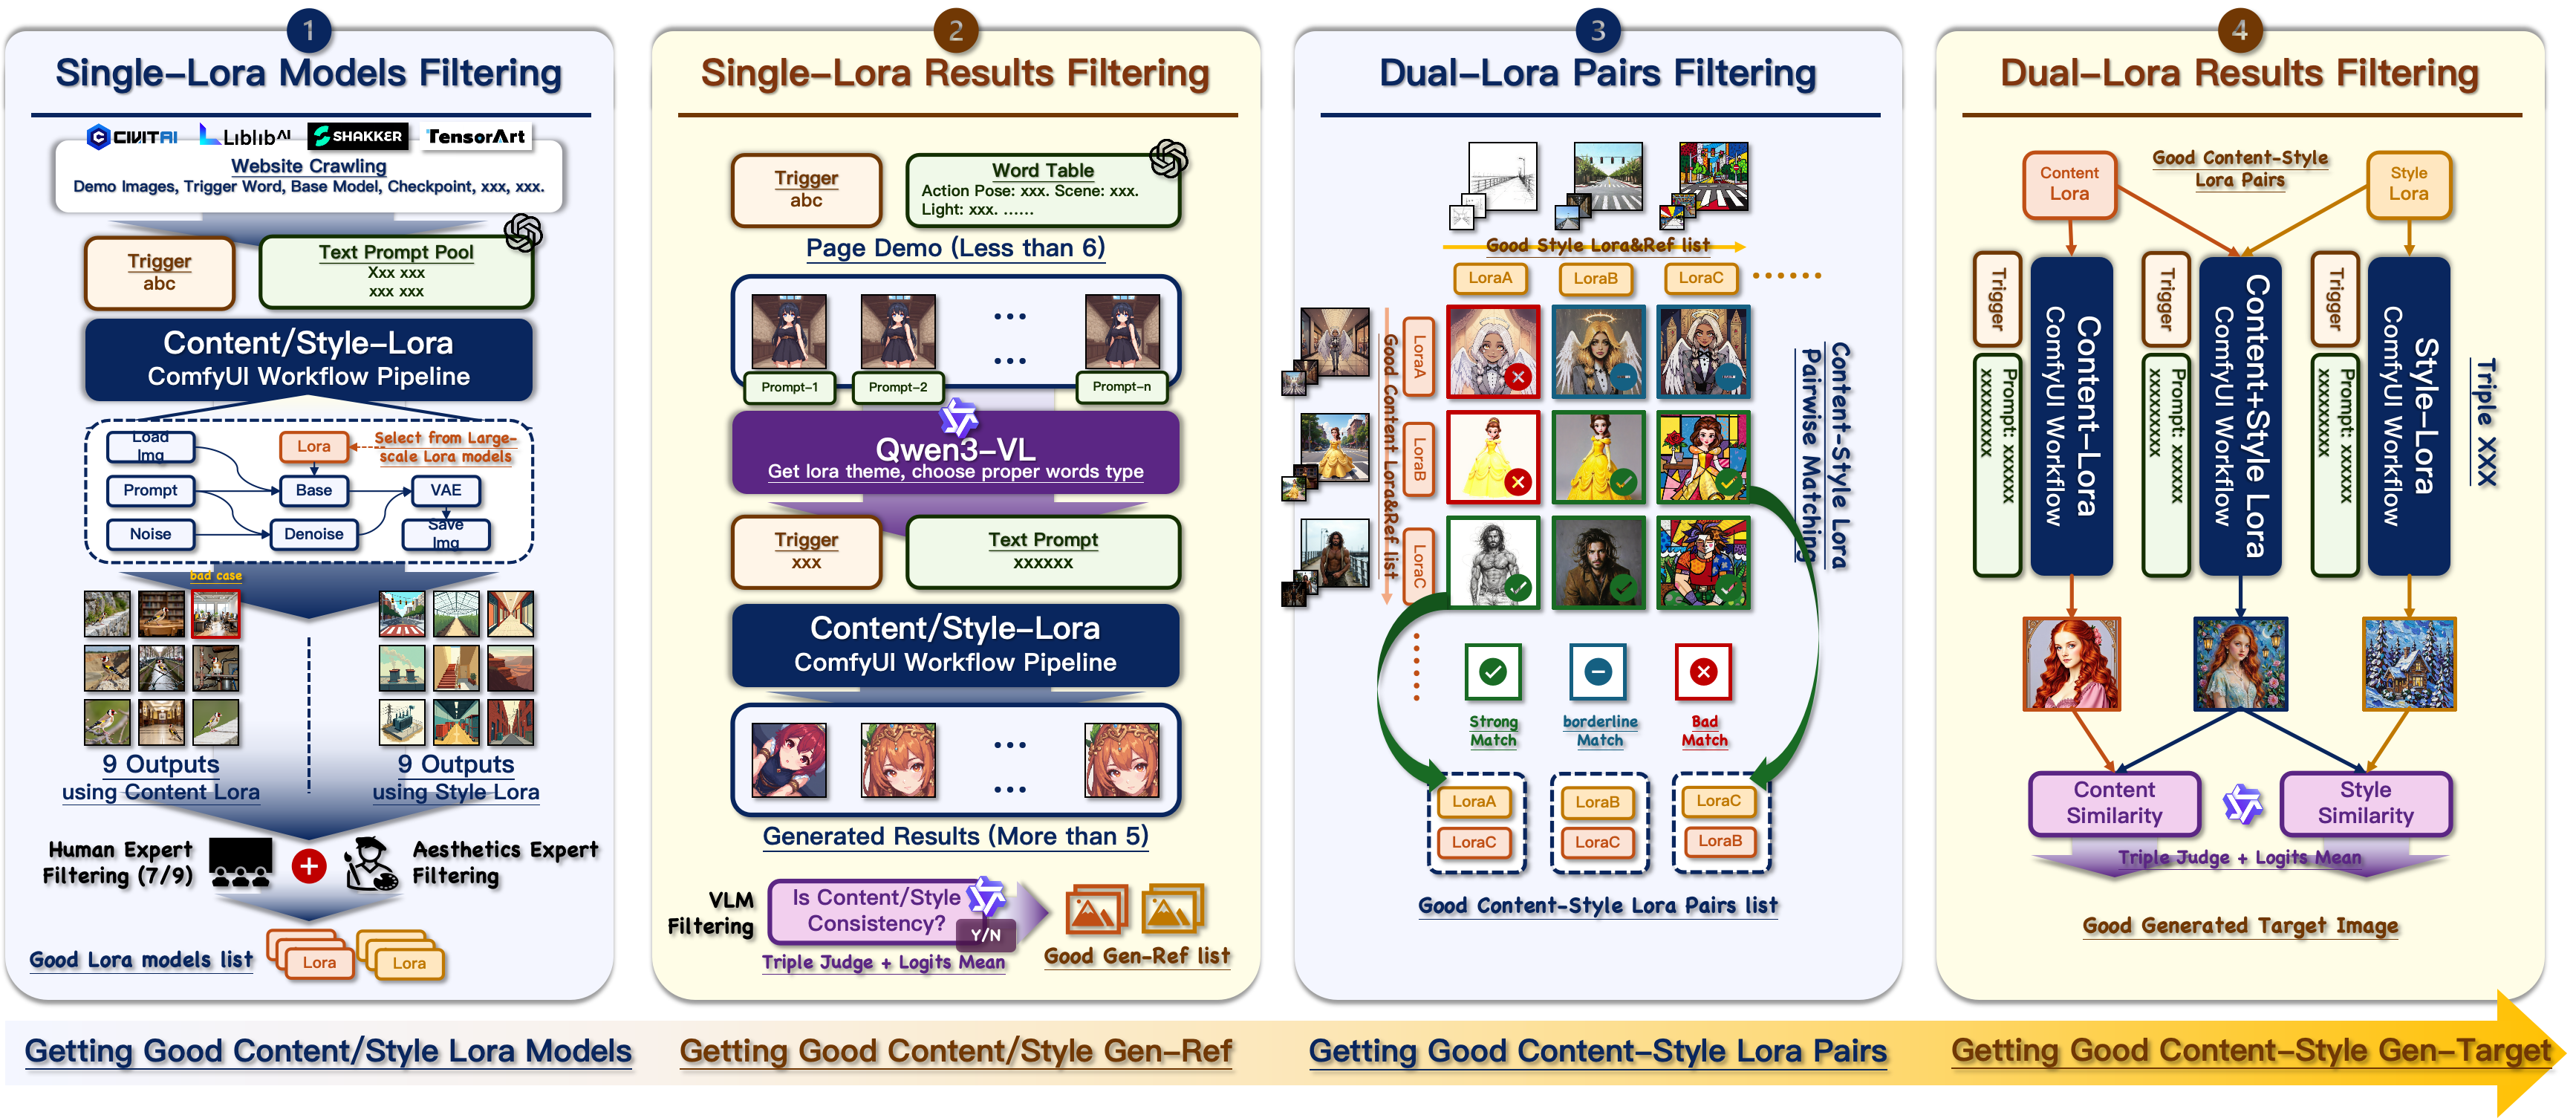
\includegraphics[width=\linewidth]{figures/VIT-TSNE/datapipeline.png}
\caption{Overview of our data pipeline.}
\label{fig:datapipeline_overview}
\end{figure}

\begin{figure}[t]
\centering
\begin{minipage}[t]{0.48\linewidth}
\centering
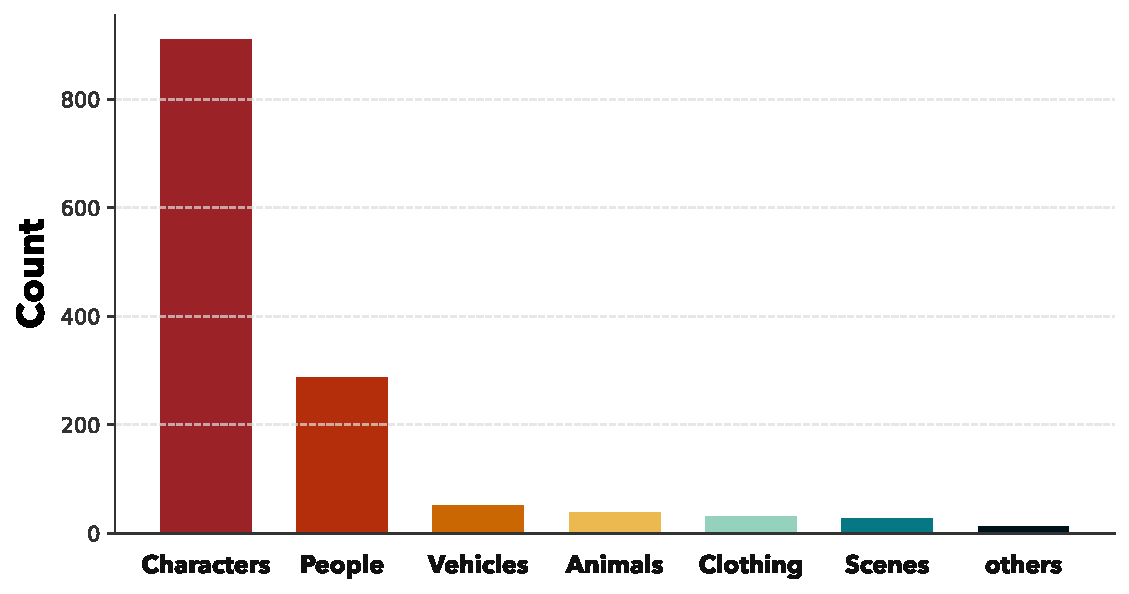
\includegraphics[height=0.28\textheight,keepaspectratio]{figures/content_category_distribution_vertical_gap15_bar1.pdf}
\end{minipage}\hfill
\begin{minipage}[t]{0.48\linewidth}
\centering
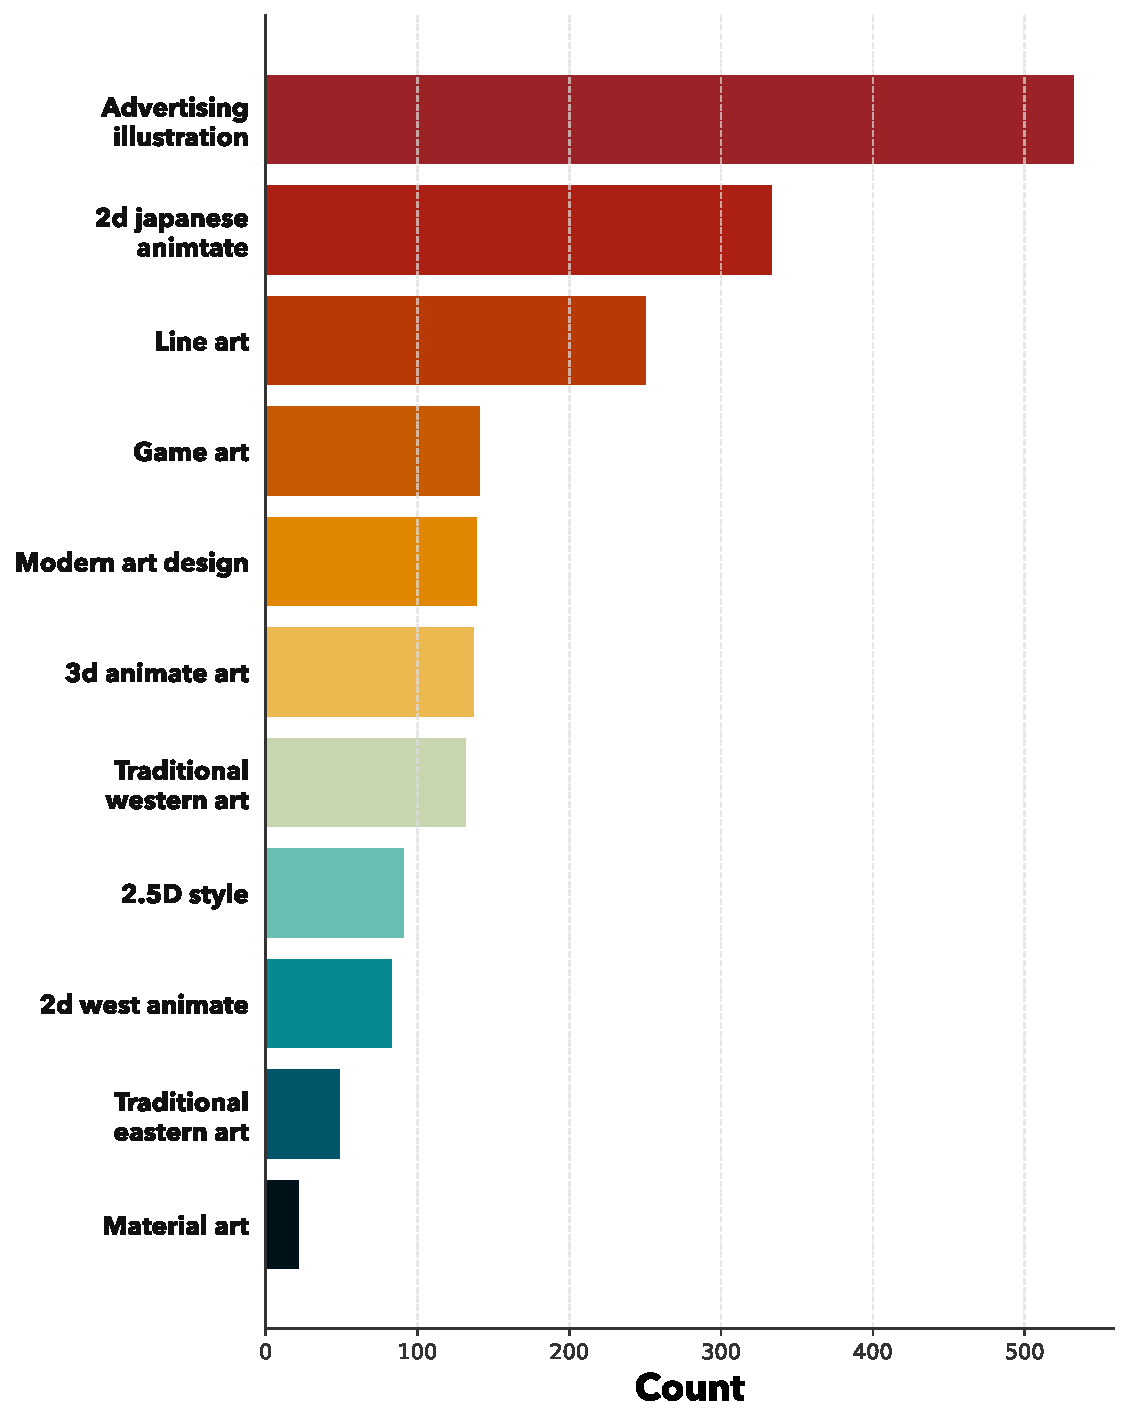
\includegraphics[height=0.28\textheight,keepaspectratio]{figures/style_category_distribution_gap15_bar1.pdf}
\end{minipage}
\caption{Distributions of mined community LoRAs across (left) content categories and (right) style categories.}
\label{fig:content_style_category_dist}
\end{figure}

To illustrate the end-to-end mining process, we provide a Sankey-style overview in Figure~\ref{fig:sankey_lora_mining}. It summarizes how the collected LoRA pool is partitioned by base model families and further filtered into content/style/unstable subsets, which are then used to construct high-quality reference triplets.
\begin{figure}[t]
\centering
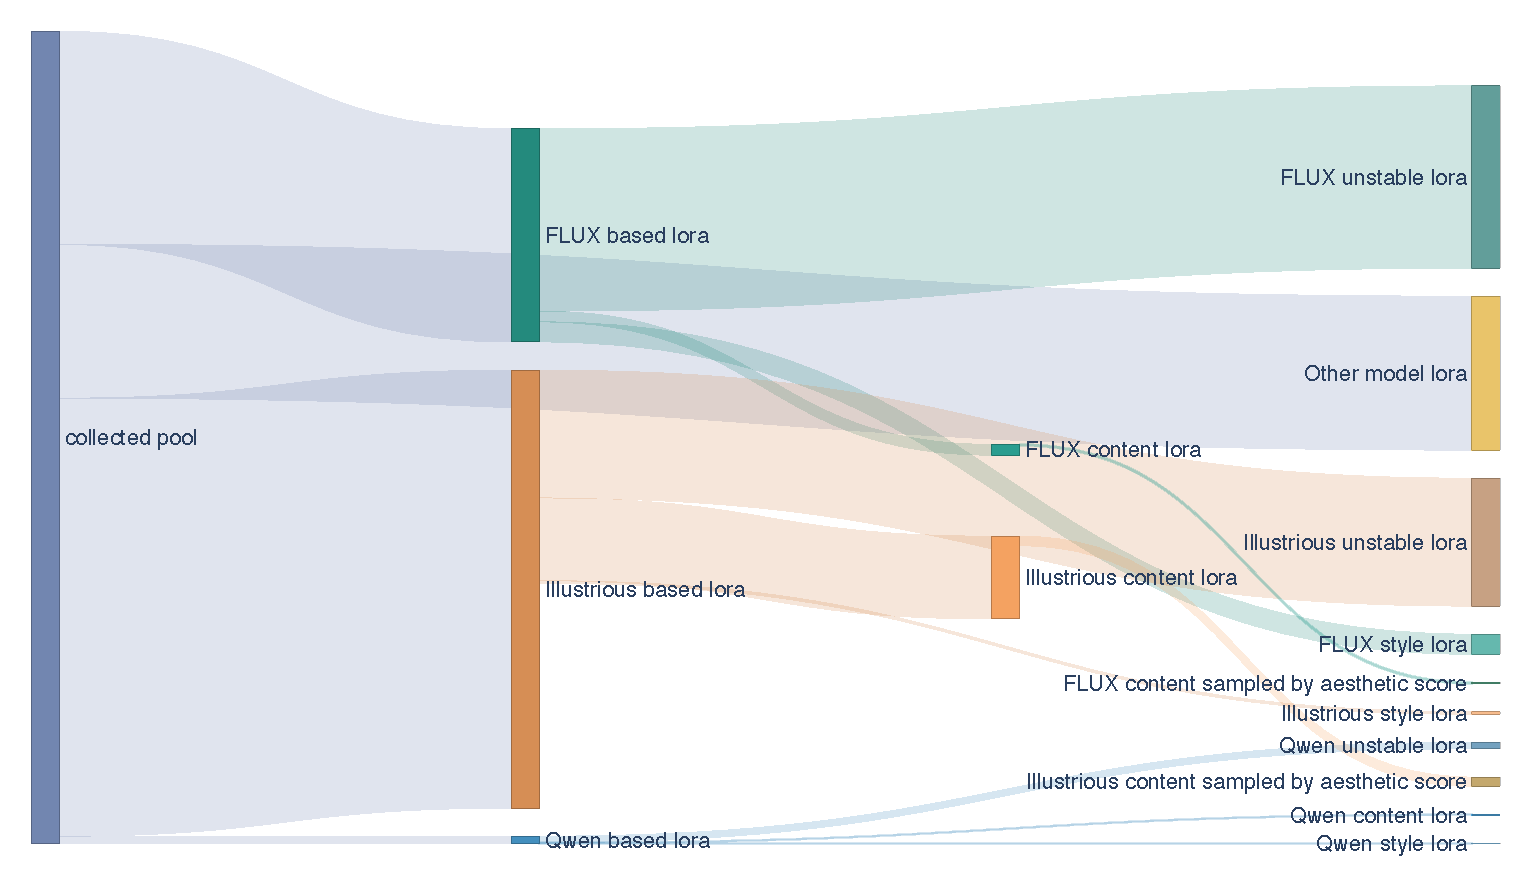
\includegraphics[width=\linewidth]{figures/sankey_lora.pdf}
\caption{Sankey diagram of our community LoRA mining and filtering pipeline.}
\label{fig:sankey_lora_mining}
\end{figure}

\begin{figure}[t]
\centering
\begin{minipage}[t]{0.68\linewidth}
\centering
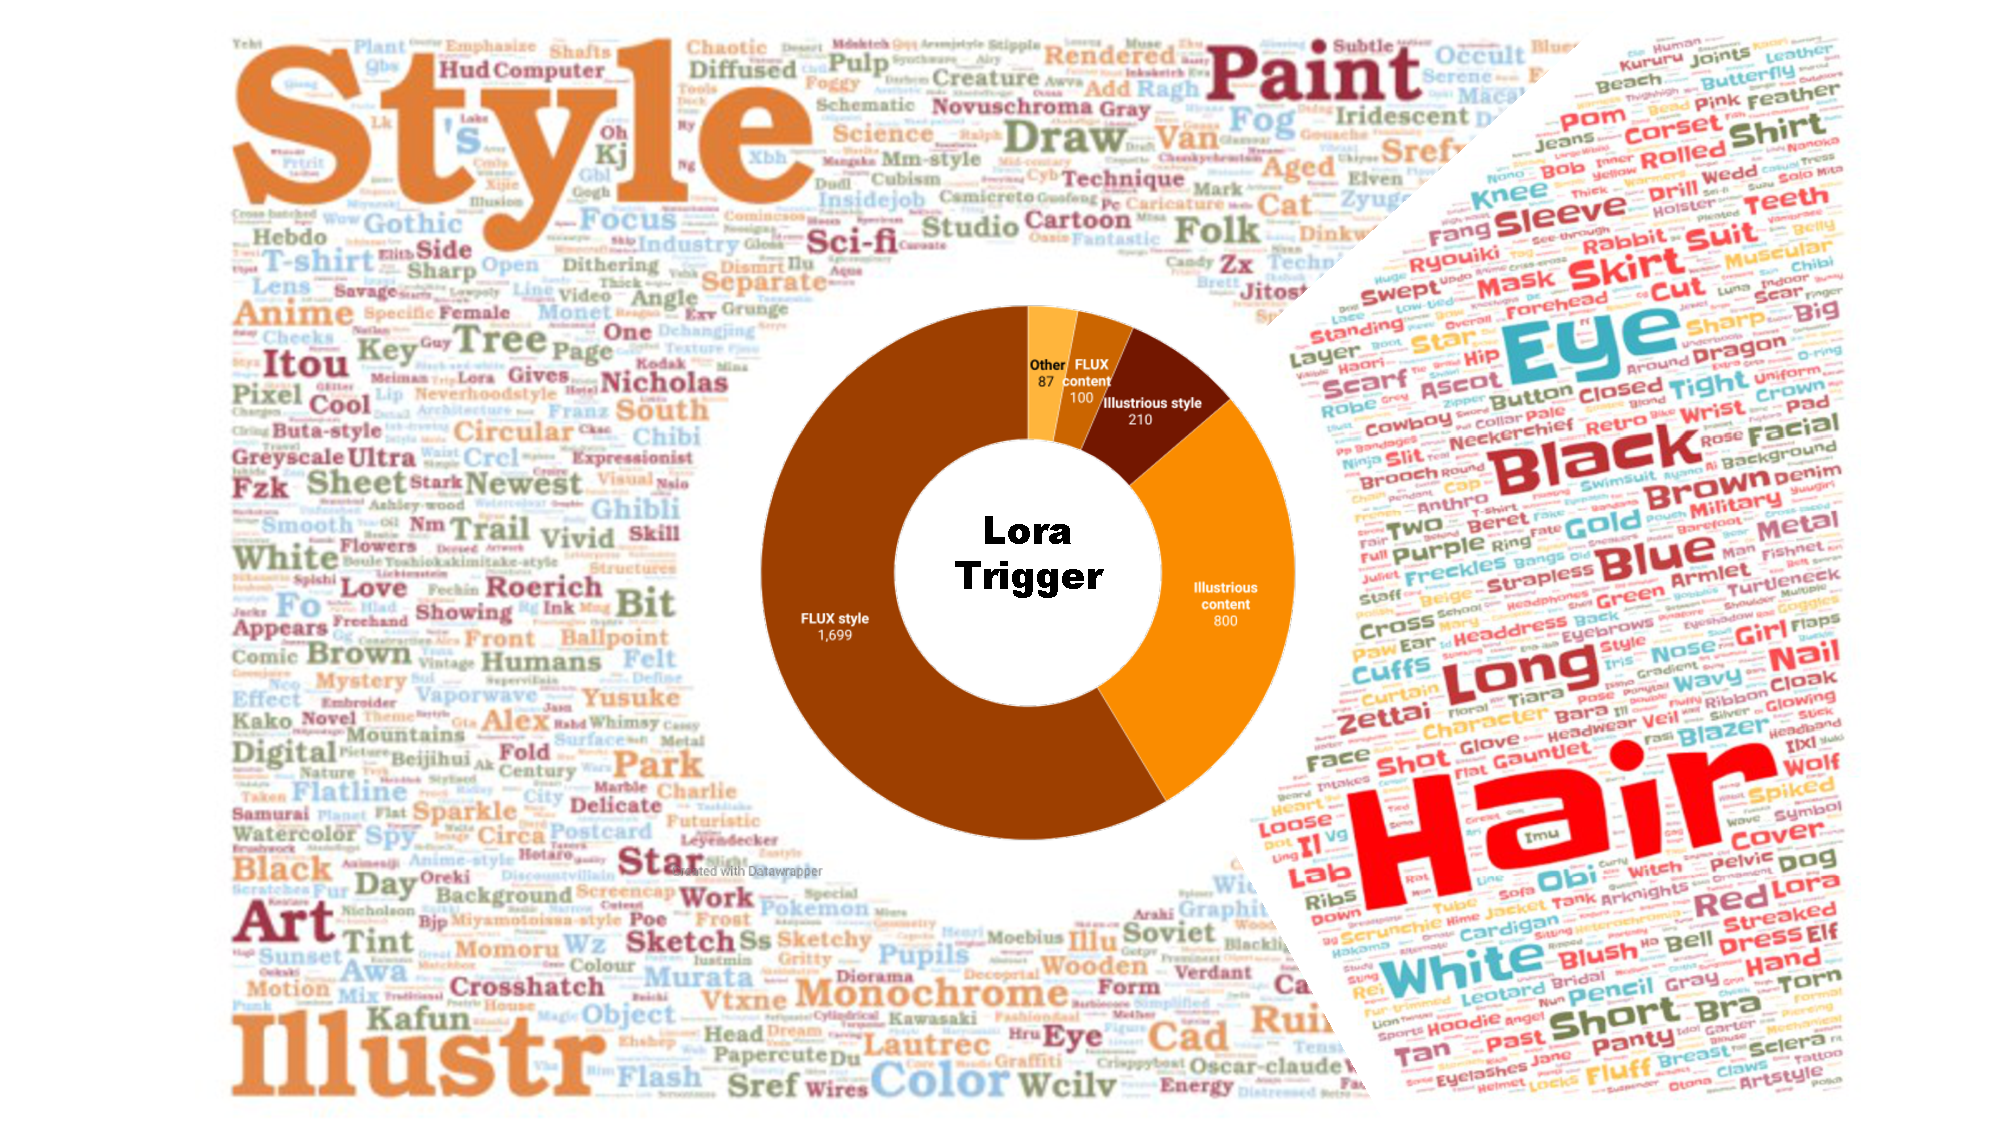
\includegraphics[width=\linewidth,height=0.24\textheight,keepaspectratio]{figures/trigger_word_dsitribution.pdf}
\end{minipage}\hfill
\begin{minipage}[t]{0.32\linewidth}
\centering
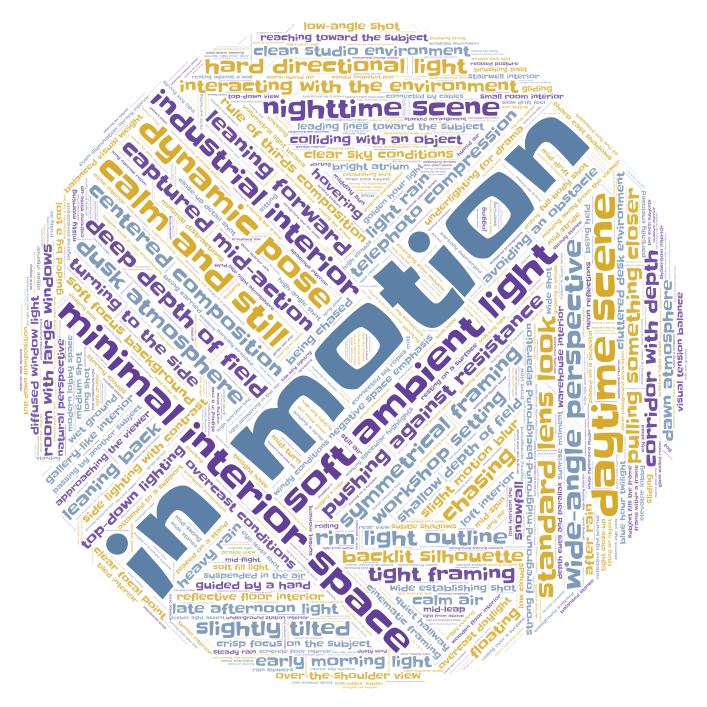
\includegraphics[width=\linewidth,height=0.24\textheight,keepaspectratio]{figures/phrase.png}
\end{minipage}
\caption{Trigger word statistics in the mined LoRA metadata (left) and a phrase word cloud (right).}
\label{fig:trigger_word_distribution}
\end{figure}


\section{benchmark}

\section{training architecture}
\subsection{image encoder insight}
%image encoder argument
%现有的image encoder对于风格图片的编码都是有损压缩，无法很好的表征出风格图像的特征，而使用DINOv2的image encoder的方法，比如USO，在Sref的任务上往往会出现风格图的内容泄漏，导致风格迁移的时候会有明显的不属于内容图的语义信息。在这方面我们做了一些可视化的实验，因此本文的图像信息在latent上还是依赖VAE编码.
Most existing image encoders provide a lossy compression of style reference images and often fail to faithfully capture fine-grained stylistic cues. In particular, approaches that rely on powerful semantic encoders such as DINOv2 (e.g., USO) can exhibit \emph{content leakage} in the style-reference setting: semantic attributes from the style image may be inadvertently injected into the output, leading to visible objects or concepts that do not belong to the content reference. Motivated by this observation, we represent image information in the VAE latent space throughout our pipeline.
%我们对一组来自illustrious basemodel的lora权重进行了推理，他们的prompt都来自于一个文本池，加上各自的触发词推理，得到风格差异大而内容差异很小的图片，经过几种常用的image encoder，最后进行t-SNE可视化，发现VAE latents能够很好的区分出不同的风格数据，而其他encoder比如其他工作常用的SigLip和DINO则无法很好的区分。

%同时我们给予illustrious的一个社区版本，waiillustrious的chekcpoint，收集了五种截然不同的风格lora，然后使用一组完全相同的prompt，加上每个lora的trigger word生成图片，将生成的图片经过不同的image encoder，发现一些image encoder无法很好的区分开不同的风格数据，尤其是CLIP-based的encoder，可能受限于他们的感知尺寸，高频纹理感知不佳。
\paragraph{Community LoRA Case Study.}
We further study a community checkpoint of Illustrious (WAI-Illustrious) and collect five stylistically distinct LoRA modules. Using an identical prompt template and each LoRA's trigger words, we generate corresponding image sets and re-encode them with different image encoders. We find that several encoders struggle to distinguish these styles, with CLIP-based encoders being particularly prone to confusion. We hypothesize this is partly due to their limited effective perceptual resolution and weaker sensitivity to high-frequency textures, which are often critical for style characterization.
\begin{figure}[t]
\centering
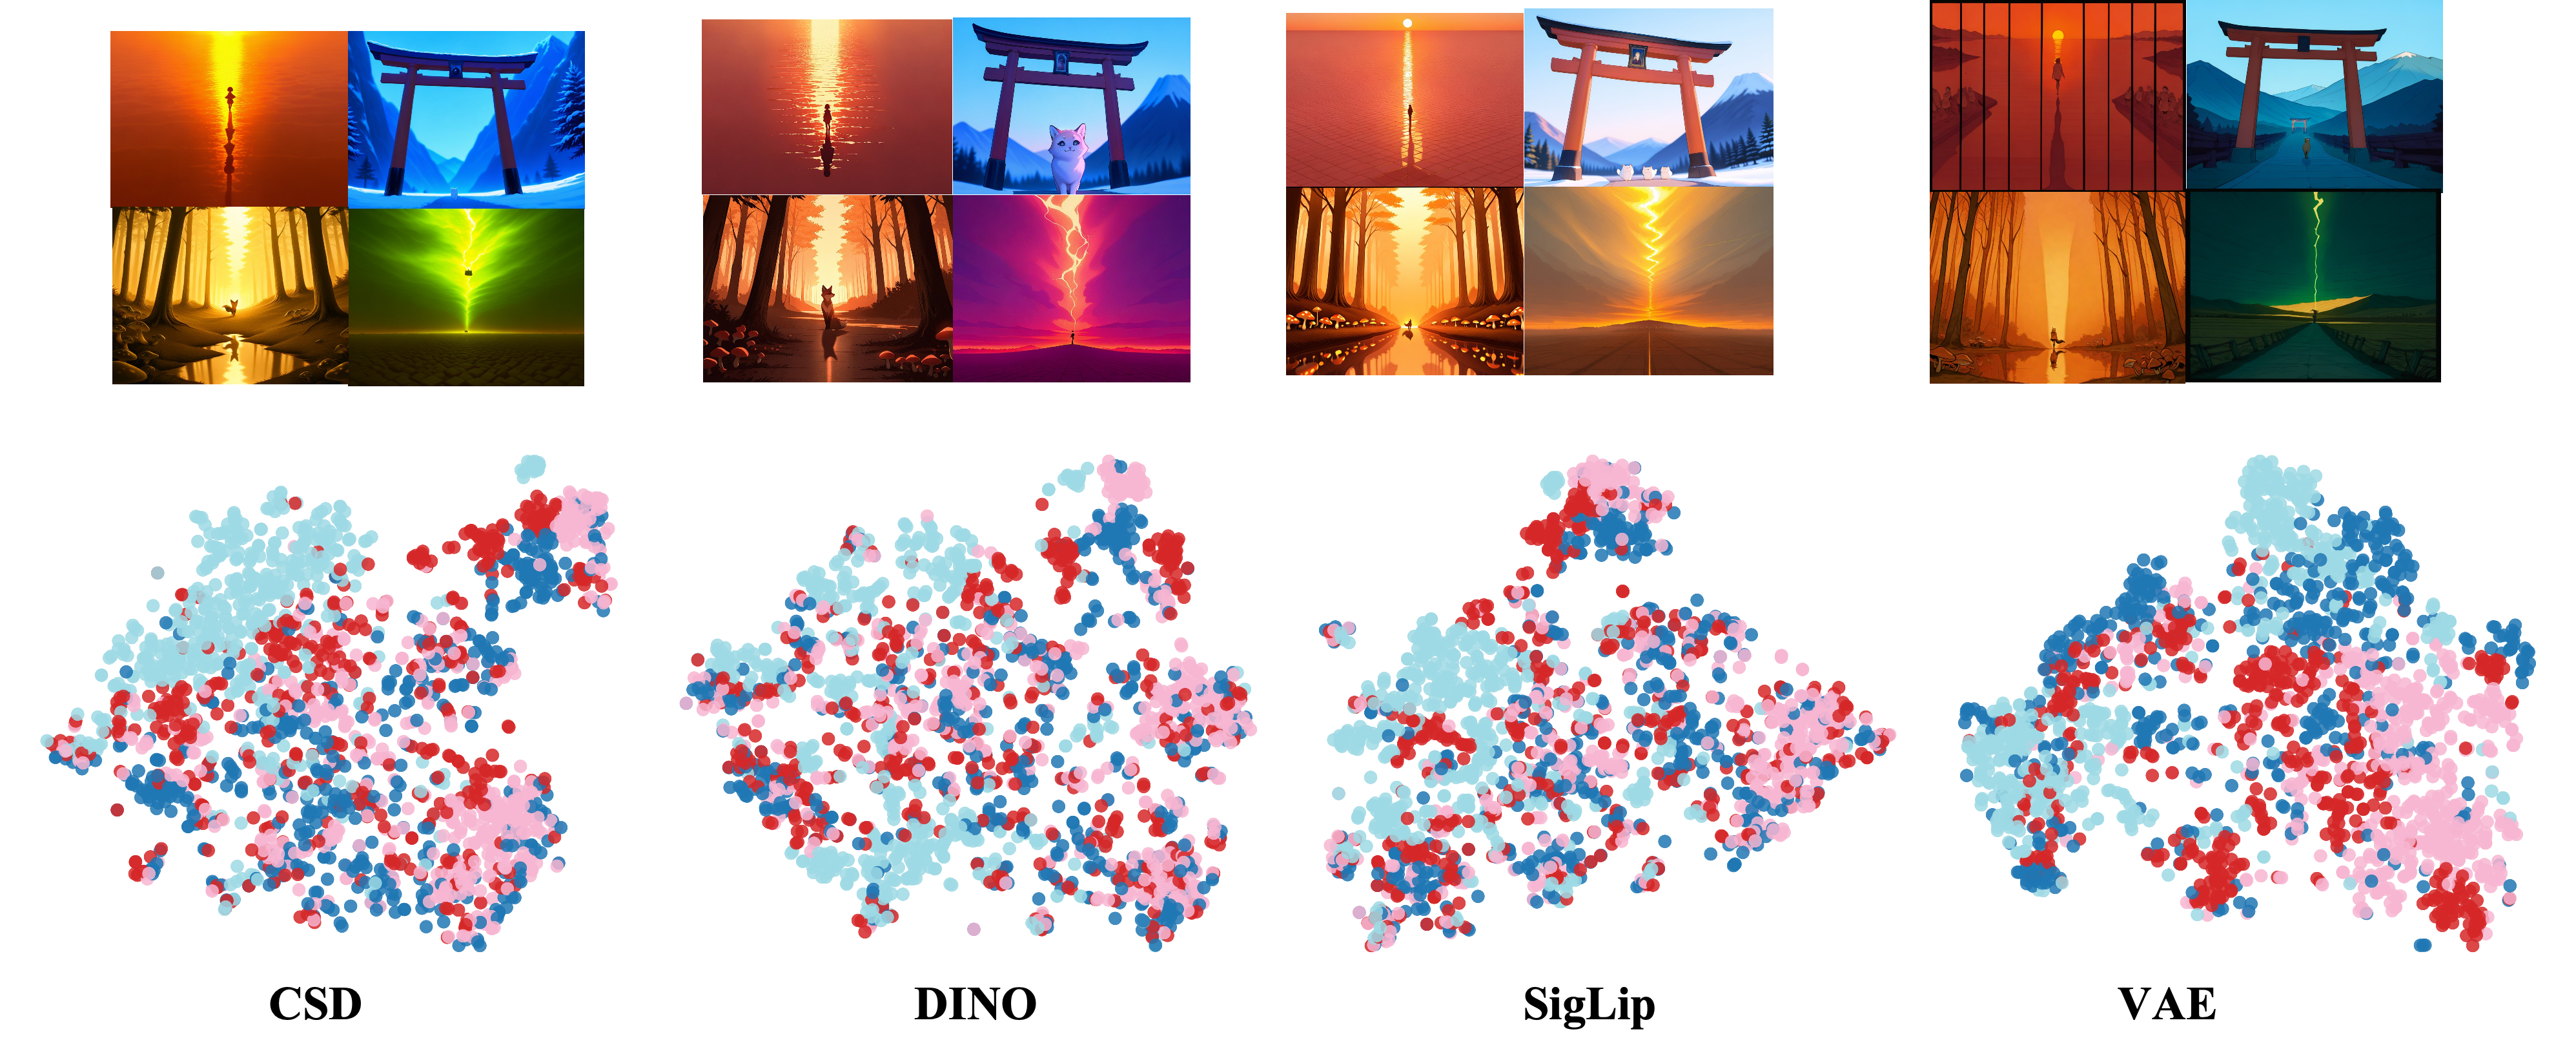
\includegraphics[width=\linewidth]{figures/VIT-TSNE/TSNE-VIT.png}
\caption{t-SNE visualization of embeddings produced by different image encoders on our collected samples.}
\label{fig:tsne_vit_encoders}
\end{figure}

\subsection{explicit content and style guidance}
%在这篇文章中我们为了避免风格图片的内容泄漏，设计了一些训练的损失函数。因为我们已经有了一个可以表征出内容和风格triplet。
%因此我们可以在训练的过程中引入损失函数，约束预测的图像要偏离风格的内容，靠近gt的内容，这样子可以显式的约束风格迁移的过程中不会出现内容泄漏的情况。
%在训练的第t步骤得到了预测的Vt，用一步推理得到x0=xt-tVt，然后计算x0和gt的内容损失，用x0和style的风格损失这个取负数，有两个参数分别加权，将这两个损失加起来，作为训练的损失函数。实现了显示的内容约束。


\begin{table}[t]
\centering
\small
\setlength{\tabcolsep}{2pt}
\renewcommand{\arraystretch}{1.15}
\begin{tabular}{@{}lrrrrrrrr@{}}
\toprule
Model & DINOv2 & CAS & ONEIG & CSD & LAION & Aes2.5 & VLM-S & VLM-C \\
\midrule
USO & 0.81 & 1.28 & 0.54 & 0.53 & 5.97 & 5.57 & 3.74 & 9.24 \\
CSGO & 0.65 & 1.66 & 0.52 & 0.67 & 5.43 & 4.68 & 6.19 & 1.52 \\
EasyRef & 0.61 & 1.90 & 0.27 & 0.58 & 5.40 & 4.42 & 2.07 & 0.43 \\
FLUX-k-9B & 0.81 & 1.08 & 0.49 & 0.66 & 6.68 & 6.02 & 6.07 & 8.34 \\
\bottomrule
\end{tabular}
\caption{Mean values of different scoring metrics across models.}
\label{tab:metric_means}
\end{table}


% ---- Bibliography ----
%
% BibTeX users should specify bibliography style 'splncs04'.
%
\bibliographystyle{splncs04}
\bibliography{main}
\end{document}
